\subsection{Chức năng bình luận}
\subsubsection{Sơ đồ use-case}
\begin{figure}[H]
    \centering
    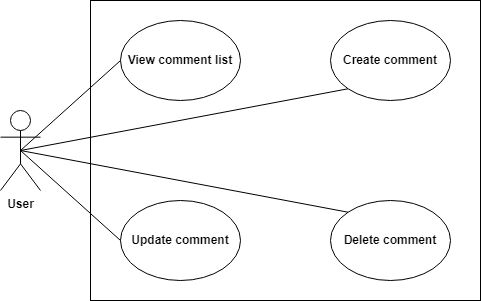
\includegraphics[width=0.7\textwidth]{Images/UseCase/Comment.png}
    \caption{Sơ đồ use-case cho các chức năng bình luận về bài đăng tải}
\end{figure}
\subsubsection{Đặc tả use-case cho chức năng xem danh sách bình luận của bài đăng tải nhà thuê}
\begin{center}
    \arrayrulecolor{cyan!75!black}
    \arrayrulewidth=2pt
    \begin{longtable}{
        |>{\raggedright\arraybackslash}p{3cm}
        |>{\raggedright\arraybackslash}p{13cm}
        |}
        \hline
        \rowcolor{cyan!75!black} \textcolor{white}{\textbf{Use-case name}} & \textcolor{white}{\textbf{XEM DANH SÁCH BÌNH LUẬN CỦA BÀI ĐĂNG TẢI}}
        \\\hline
        \rowcolor{cyan!10!white} \textit{Actor} & Người dùng
        \\\hdashline
        \rowcolor{cyan!10!white} \textit{Description} & Tính năng cho phép người dùng xem được danh sách các bình luận và các phản hồi cho từng bình luận cho một bài đăng tải nhà thuê nhất định.
        \\\hdashline
        \rowcolor{cyan!10!white} \textit{Preconditions} & Không có.
        \\\hdashline
        \rowcolor{cyan!10!white} \textit{Postconditions} & Kết quả được trả về thành công dưới dạng danh sách các bình luận kèm theo các phản hồi của từng bình luận cho một bài đăng tải nhà thuê nhất định.
        \\\hdashline
        \rowcolor{cyan!10!white} \textit{Trigger} & Người dùng nhấn vào một bài đăng tải nhà thuê nhất định, sau đó kéo xuống phía dưới ở mục bình luận.
        \\\hdashline
        \rowcolor{cyan!10!white} \textit{Main flow} &
        1. Người dùng truy cập vào mục bình luận ở thông tin bài đăng tải nhà thuê. \newline
        2. Ứng dụng truy vấn danh sách các bình luận đối với bài đăng tải nhà thuê đó. \newline
        3. Kết quả danh sách các bình luận kèm theo các phản hồi cho từng bình luận cho bài đăng tải nhà thuê được hiển thị thành công trên giao diện.
        \\\hdashline
        \rowcolor{cyan!10!white} \textit{Alternative flow} & Không có
        \\\hdashline
        \rowcolor{cyan!10!white} \textit{Exception flow} &
        \textbf{Nếu ứng dụng gặp lỗi khi thực hiện lấy ra danh sách các bình luận của bài đăng tải nhà thuê, ứng dụng thông báo lỗi và yêu cầu người dùng thử lại sau} \newline
        1a.1. Ứng dụng hiện lỗi khi thực hiện lấy ra danh sách các bình luận của bài đăng tải nhà thuê. \newline
        1a.2. Ứng dụng thông báo yêu cầu người dùng thử lại sau.
        \\\hline
        \caption{Đặc tả use-case cho chức năng xem danh sách các bình luận của bài đăng tải nhà thuê}
    \end{longtable}
\end{center}
\subsubsection{Đặc tả use-case cho chức năng tạo bình luận mới cho bài đăng tải nhà thuê}
\begin{center}
    \arrayrulecolor{cyan!75!black}
    \arrayrulewidth=2pt
    \begin{longtable}{
        |>{\raggedright\arraybackslash}p{3cm}
        |>{\raggedright\arraybackslash}p{13cm}
        |}
        \hline
        \rowcolor{cyan!75!black} \textcolor{white}{\textbf{Use-case name}} & \textcolor{white}{\textbf{TẠO BÌNH LUẬN MỚI CHO BÀI ĐĂNG TẢI NHÀ THUÊ}}
        \\\hline
        \rowcolor{cyan!10!white} \textit{Actor} & Người dùng
        \\\hdashline
        \rowcolor{cyan!10!white} \textit{Description} & Tính năng cho phép người dùng tạo mới một bình luận đối với một bài đăng tải nhà thuê nhất định.
        \\\hdashline
        \rowcolor{cyan!10!white} \textit{Preconditions} & Người dùng đã đăng nhập thành công vào ứng dụng.
        \\\hdashline
        \rowcolor{cyan!10!white} \textit{Postconditions} & Bình luận cho bài đăng tải nhà thuê được ghi nhận thành công.
        \\\hdashline
        \rowcolor{cyan!10!white} \textit{Trigger} & Người dùng chọn vào mục \textbf{Thêm bình luận} ở trên giao diện thông tin chi tiết bài đăng tải nhà thuê.
        \\\hdashline
        \rowcolor{cyan!10!white} \textit{Main flow} &
        1. Ứng dụng hiển thị các trường thông tin yêu cầu người dùng cung cấp khi tạo bình luận cho bài đăng tải nhà thuê. \newline
        2. Người dùng nhập vào các trường thông tin cho một bình luận, bao gồm nội dung và đánh giá số sao. \newline
        3. Người dùng nhấn vào mục \textbf{Tạo bình luận}. \newline
        4. Ứng dụng kiểm tra và xử lý các trường thông tin do người dùng cung cấp. \newline
        5. Ứng dụng thông báo đăng tải bình luận thành công.
        \\\hdashline
        \rowcolor{cyan!10!white} \textit{Alternative flow} & 
        \textbf{Nếu người dùng hủy đăng tải bình luận, ứng dụng sẽ quay trở lại giao diện chính} \newline
        2a.1. Người dùng hủy quá trình đăng tải bình luận. \newline
        2a.2. Ứng dụng quay trở lại giao diện chính.
        \\\hdashline
        \rowcolor{cyan!10!white} \textit{Exception flow} & 
        \textbf{Nếu thông tin bình luận không được cung cấp đầy đủ, ứng dụng sẽ hiển thị lỗi và yêu cầu người dùng cung cấp lại thông tin} \newline
        4a.1. Ứng dụng thông báo thông tin của bình luận chưa đầy đủ. \newline
        4a.2. Người dùng bổ sung thông tin cho bình luận. \newline
        4a.3. Ứng dụng kiểm tra thông tin đã nhập. \newline
        4a.4. Nếu thông tin hợp lệ, ứng dụng sẽ thông báo đăng tải bình luận thành công, ngược lại sẽ quay lại bước 2. \newline
        \textbf{Nếu thông tin đăng tải bình luận không hợp lệ, ứng dụng sẽ hiển thị lỗi và yêu cầu người dùng cung cấp lại thông tin} \newline
        4a.1. Ứng dụng thông báo thông tin của bình luận không hợp lệ. \newline
        4a.2. Người dùng chỉnh sửa thông tin bình luận. \newline
        4a.3. Ứng dụng kiểm tra thông tin đã nhập. \newline
        4a.4. Nếu thông tin hợp lệ, ứng dụng sẽ thông báo đăng tải bình luận thành công, ngược lại sẽ quay lại bước 2. \newline
        \textbf{Nếu ứng dụng gặp lỗi trong quá trình đăng tải bình luận, ứng dụng thông báo lỗi và yêu cầu người dùng thử lại sau} \newline
        4c.1. Ứng dụng hiện lỗi khi thực hiện đăng tải bình luận. \newline
        4c.2. Ứng dụng thông báo yêu cầu người dùng thử lại sau.
        \\\hline
        \caption{Đặc tả use-case cho chức năng tạo bình luận mới cho bài đăng tải nhà thuê}
    \end{longtable}
\end{center}
\subsubsection{Đặc tả use-case cho chức năng chỉnh sửa bình luận cho bài đăng tải nhà thuê}
\begin{center}
    \arrayrulecolor{cyan!75!black}
    \arrayrulewidth=2pt
    \begin{longtable}{
        |>{\raggedright\arraybackslash}p{3cm}
        |>{\raggedright\arraybackslash}p{13cm}
        |}
        \hline
        \rowcolor{cyan!75!black} \textcolor{white}{\textbf{Use-case name}} & \textcolor{white}{\textbf{CHỈNH SỬA BÌNH LUẬN CHO BÀI ĐĂNG TẢI NHÀ THUÊ}}
        \\\hline
        \rowcolor{cyan!10!white} \textit{Actor} & Người dùng
        \\\hdashline
        \rowcolor{cyan!10!white} \textit{Description} & Tính năng cho phép người dùng chỉnh sửa một bình luận có sẵn của người dùng đối với một bài đăng tải nhà thuê nhất định.
        \\\hdashline
        \rowcolor{cyan!10!white} \textit{Preconditions} & Người dùng đã đăng nhập thành công vào ứng dụng. Người dùng có ít nhất một bình luận đối với một bài đăng tải nhà thuê nhất định.
        \\\hdashline
        \rowcolor{cyan!10!white} \textit{Postconditions} & Bình luận cho bài đăng tải nhà thuê được cập nhật thành công.
        \\\hdashline
        \rowcolor{cyan!10!white} \textit{Trigger} & Người dùng chọn vào mục \textbf{Chỉnh sửa bình luận} ở phần bình luận của người dùng.
        \\\hdashline
        \rowcolor{cyan!10!white} \textit{Main flow} &
        1. Ứng dụng hiển thị các trường thông tin hiện tại của bình luận của người dùng cho bài đăng tải nhà thuê. \newline
        2. Người dùng nhập vào các trường thông tin muốn thay đổi cho một bình luận, bao gồm nội dung và đánh giá số sao. \newline
        3. Người dùng nhấn vào mục \textbf{Cập nhật bình luận}. \newline
        4. Ứng dụng kiểm tra và xử lý các trường thông tin do người dùng cung cấp. \newline
        5. Ứng dụng thông báo cập nhật bình luận thành công.
        \\\hdashline
        \rowcolor{cyan!10!white} \textit{Alternative flow} & 
        \textbf{Nếu người dùng hủy cập nhật bình luận, ứng dụng sẽ quay trở lại giao diện chính} \newline
        2a.1. Người dùng hủy quá trình cập nhật bình luận. \newline
        2a.2. Ứng dụng quay trở lại giao diện chính.
        \\\hdashline
        \rowcolor{cyan!10!white} \textit{Exception flow} & 
        \textbf{Nếu thông tin bình luận bị bỏ trống, ứng dụng sẽ hiển thị lỗi và yêu cầu người dùng cung cấp lại thông tin} \newline
        4a.1. Ứng dụng thông báo thông tin của bình luận bị bỏ trống. \newline
        4a.2. Người dùng bổ sung thông tin cho bình luận. \newline
        4a.3. Ứng dụng kiểm tra thông tin đã nhập. \newline
        4a.4. Nếu thông tin hợp lệ, ứng dụng sẽ thông báo cập nhật bình luận thành công, ngược lại sẽ quay lại bước 2. \newline
        \textbf{Nếu thông tin cập nhật cho bình luận không hợp lệ, ứng dụng sẽ hiển thị lỗi và yêu cầu người dùng cung cấp lại thông tin} \newline
        4a.1. Ứng dụng thông báo thông tin cập nhật bình luận không hợp lệ. \newline
        4a.2. Người dùng chỉnh sửa thông tin bình luận. \newline
        4a.3. Ứng dụng kiểm tra thông tin đã nhập. \newline
        4a.4. Nếu thông tin hợp lệ, ứng dụng sẽ thông báo cập nhật bình luận thành công, ngược lại sẽ quay lại bước 2. \newline
        \textbf{Nếu ứng dụng gặp lỗi trong quá trình cập nhật bình luận, ứng dụng thông báo lỗi và yêu cầu người dùng thử lại sau} \newline
        4c.1. Ứng dụng hiện lỗi khi thực hiện cập nhật bình luận. \newline
        4c.2. Ứng dụng thông báo yêu cầu người dùng thử lại sau.
        \\\hline
        \caption{Đặc tả use-case cho chức năng chỉnh sửa bình luận cho bài đăng tải nhà thuê}
    \end{longtable}
\end{center}
\subsubsection{Đặc tả use-case cho chức năng xóa bình luận cho bài đăng tải nhà thuê}
\begin{center}
    \arrayrulecolor{cyan!75!black}
    \arrayrulewidth=2pt
    \begin{longtable}{
        |>{\raggedright\arraybackslash}p{3cm}
        |>{\raggedright\arraybackslash}p{13cm}
        |}
        \hline
        \rowcolor{cyan!75!black} \textcolor{white}{\textbf{Use-case name}} & \textcolor{white}{\textbf{XÓA BÌNH LUẬN CHO BÀI ĐĂNG TẢI NHÀ THUÊ}}
        \\\hline
        \rowcolor{cyan!10!white} \textit{Actor} & Người dùng
        \\\hdashline
        \rowcolor{cyan!10!white} \textit{Description} & Tính năng cho phép người dùng xóa một bình luận của bài đăng tải cho thuê nhà.
        \\\hdashline
        \rowcolor{cyan!10!white} \textit{Preconditions} & Người dùng đã đăng nhập thành công vào ứng dụng. Người dùng đã có ít nhất một bình luận trên một bài đăng tải nhà thuê trên ứng dụng.
        \\\hdashline
        \rowcolor{cyan!10!white} \textit{Postconditions} & Bình luận của người dùng được xóa thành công.
        \\\hdashline
        \rowcolor{cyan!10!white} \textit{Trigger} & Người dùng chọn vào một bình luận nhất định do người dùng đó đăng tải và chọn mục \textbf{Xóa bình luận}.
        \\\hdashline
        \rowcolor{cyan!10!white} \textit{Main flow} &
        1. Ứng dụng hiển thị bình luận hiện tại của người dùng. \newline
        3. Người dùng nhấn vào mục \textbf{Xóa bình luận}. \newline
        4. Ứng dụng yêu cầu người dùng xác nhận việc xóa bình luận. \newline
        5. Người dùng xác nhận việc xóa bình luận. \newline
        6. Ứng dụng thông báo xóa bình luận thành công.
        \\\hdashline
        \rowcolor{cyan!10!white} \textit{Alternative flow} & 
        \textbf{Nếu người dùng hủy xóa bình luận, ứng dụng sẽ quay trở lại giao diện chính} \newline
        2a.1. Người dùng hủy quá trình xóa bình luận. \newline
        2a.2. Ứng dụng quay trở lại giao diện chính.
        \\\hdashline
        \rowcolor{cyan!10!white} \textit{Exception flow} & 
        \textbf{Nếu ứng dụng gặp lỗi trong quá trình xóa bình luận, ứng dụng thông báo lỗi và yêu cầu người dùng thử lại sau} \newline
        4c.1. Ứng dụng hiện lỗi khi thực hiện xóa bình luận. \newline
        4c.2. Ứng dụng thông báo yêu cầu người dùng thử lại sau.
        \\\hline
        \caption{Đặc tả use-case cho chức năng xóa bình luận cho bài đăng tải nhà thuê}
    \end{longtable}
\end{center}